\documentclass[14pt]{extbook}
\usepackage{multicol, enumerate, enumitem, hyperref, color, soul, setspace, parskip, fancyhdr} %General Packages
\usepackage{amssymb, amsthm, amsmath, latexsym, units, mathtools} %Math Packages
\everymath{\displaystyle} %All math in Display Style
% Packages with additional options
\usepackage[headsep=0.5cm,headheight=12pt, left=1 in,right= 1 in,top= 1 in,bottom= 1 in]{geometry}
\usepackage[usenames,dvipsnames]{xcolor}
\usepackage{dashrule}  % Package to use the command below to create lines between items
\newcommand{\litem}[1]{\item#1\hspace*{-1cm}\rule{\textwidth}{0.4pt}}
\pagestyle{fancy}
\lhead{Makeup Progress Quiz 2}
\chead{}
\rhead{Version B}
\lfoot{2790-1423}
\cfoot{}
\rfoot{Summer C 2021}
\begin{document}

\begin{enumerate}
\litem{
Choose the graph of the equation below.\[ f(x) = \frac{-1}{x - 3} + 3 \]\begin{enumerate}[label=\Alph*.]
\begin{multicols}{2}\item 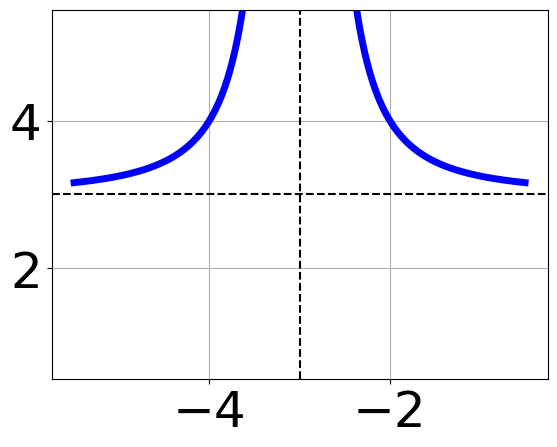
\includegraphics[width = 0.3\textwidth]{../Figures/rationalEquationToGraphAB.png}\item 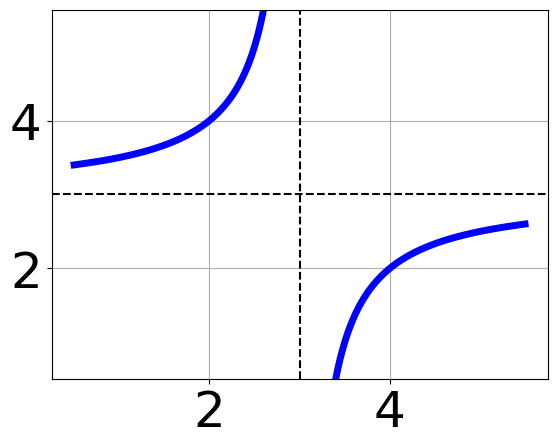
\includegraphics[width = 0.3\textwidth]{../Figures/rationalEquationToGraphBB.png}\item 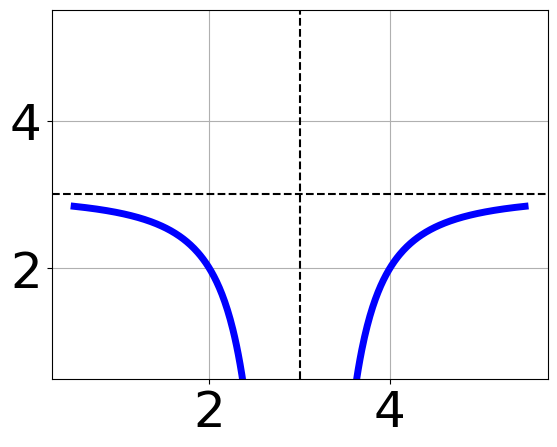
\includegraphics[width = 0.3\textwidth]{../Figures/rationalEquationToGraphCB.png}\item 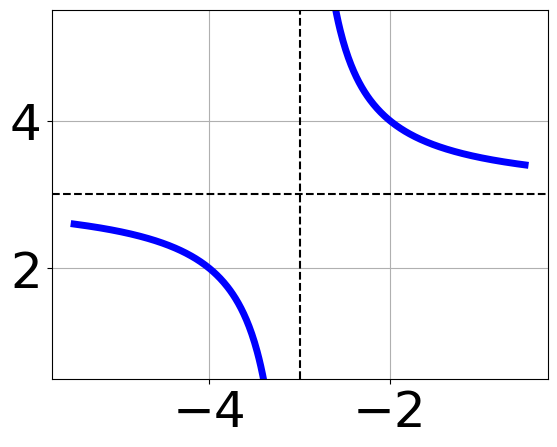
\includegraphics[width = 0.3\textwidth]{../Figures/rationalEquationToGraphDB.png}\end{multicols}\item None of the above.
\end{enumerate} }
\litem{
Solve the rational equation below. Then, choose the interval(s) that the solution(s) belongs to.\[ \frac{98}{-42x + 70} + 1 = \frac{98}{-42x + 70} \]\begin{enumerate}[label=\Alph*.]
\item \( x_1 \in [-2.67, 0.33] \text{ and } x_2 \in [-0.33,2.67] \)
\item \( x \in [-2.67,0.33] \)
\item \( \text{All solutions lead to invalid or complex values in the equation.} \)
\item \( x \in [0.67,2.67] \)
\item \( x_1 \in [0.67, 2.67] \text{ and } x_2 \in [-0.33,2.67] \)

\end{enumerate} }
\litem{
Choose the graph of the equation below.\[ f(x) = \frac{1}{x - 1} - 1 \]\begin{enumerate}[label=\Alph*.]
\begin{multicols}{2}\item 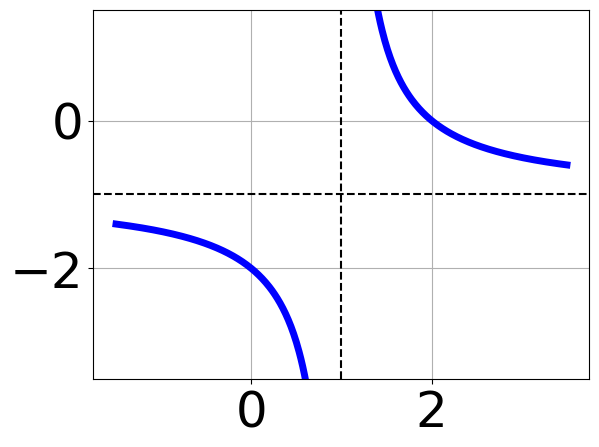
\includegraphics[width = 0.3\textwidth]{../Figures/rationalEquationToGraphCopyAB.png}\item 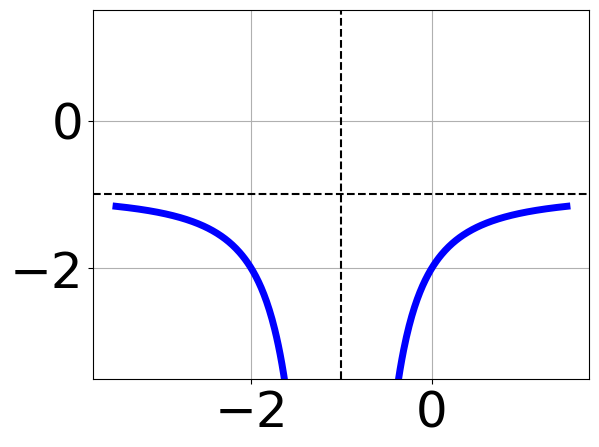
\includegraphics[width = 0.3\textwidth]{../Figures/rationalEquationToGraphCopyBB.png}\item 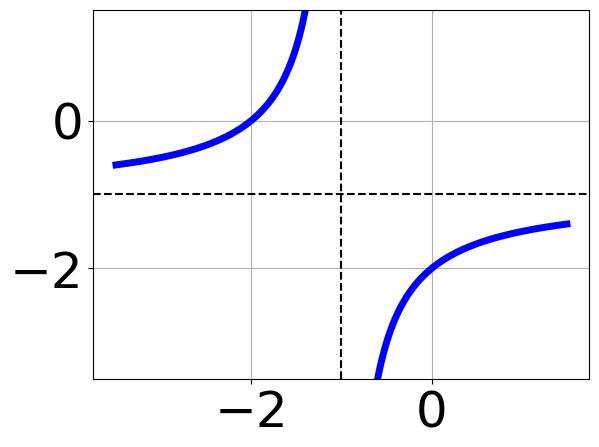
\includegraphics[width = 0.3\textwidth]{../Figures/rationalEquationToGraphCopyCB.png}\item 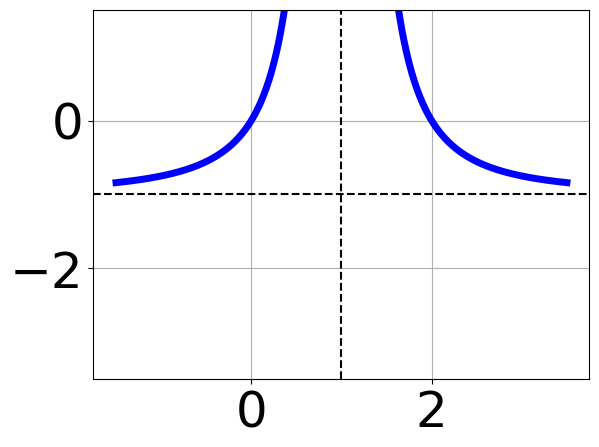
\includegraphics[width = 0.3\textwidth]{../Figures/rationalEquationToGraphCopyDB.png}\end{multicols}\item None of the above.
\end{enumerate} }
\litem{
Solve the rational equation below. Then, choose the interval(s) that the solution(s) belongs to.\[ \frac{3}{-8x + 3} + -4 = \frac{9}{64x -24} \]\begin{enumerate}[label=\Alph*.]
\item \( \text{All solutions lead to invalid or complex values in the equation.} \)
\item \( x \in [0.25,2.25] \)
\item \( x \in [-1.3,-0.2] \)
\item \( x_1 \in [-1.3, -0.2] \text{ and } x_2 \in [0.16,0.37] \)
\item \( x_1 \in [0, 0.6] \text{ and } x_2 \in [0.49,0.57] \)

\end{enumerate} }
\litem{
Determine the domain of the function below.\[ f(x) = \frac{5}{18x^{2} -33 x + 15} \]\begin{enumerate}[label=\Alph*.]
\item \( \text{All Real numbers except } x = a, \text{ where } a \in [0.65, 0.85] \)
\item \( \text{All Real numbers except } x = a \text{ and } x = b, \text{ where } a \in [8.93, 9.23] \text{ and } b \in [29.76, 30.07] \)
\item \( \text{All Real numbers.} \)
\item \( \text{All Real numbers except } x = a, \text{ where } a \in [8.93, 9.23] \)
\item \( \text{All Real numbers except } x = a \text{ and } x = b, \text{ where } a \in [0.65, 0.85] \text{ and } b \in [0.85, 1.05] \)

\end{enumerate} }
\litem{
Choose the equation of the function graphed below.
\begin{center}
    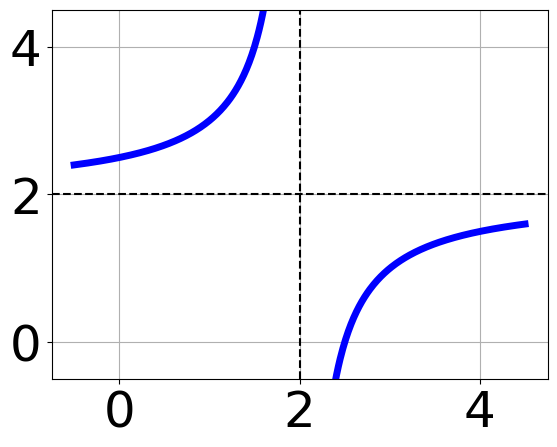
\includegraphics[width=0.5\textwidth]{../Figures/rationalGraphToEquationB.png}
\end{center}
\begin{enumerate}[label=\Alph*.]
\item \( f(x) = \frac{1}{x - 2} + 0 \)
\item \( f(x) = \frac{-1}{x + 2} + 0 \)
\item \( f(x) = \frac{1}{(x - 2)^2} + 0 \)
\item \( f(x) = \frac{-1}{(x + 2)^2} + 0 \)
\item \( \text{None of the above} \)

\end{enumerate} }
\litem{
Determine the domain of the function below.\[ f(x) = \frac{6}{9x^{2} +9 x -18} \]\begin{enumerate}[label=\Alph*.]
\item \( \text{All Real numbers.} \)
\item \( \text{All Real numbers except } x = a \text{ and } x = b, \text{ where } a \in [-2.2, -1.9] \text{ and } b \in [0.5, 3.3] \)
\item \( \text{All Real numbers except } x = a, \text{ where } a \in [-2.2, -1.9] \)
\item \( \text{All Real numbers except } x = a \text{ and } x = b, \text{ where } a \in [-19.1, -16.9] \text{ and } b \in [8.3, 10.9] \)
\item \( \text{All Real numbers except } x = a, \text{ where } a \in [-19.1, -16.9] \)

\end{enumerate} }
\litem{
Choose the equation of the function graphed below.
\begin{center}
    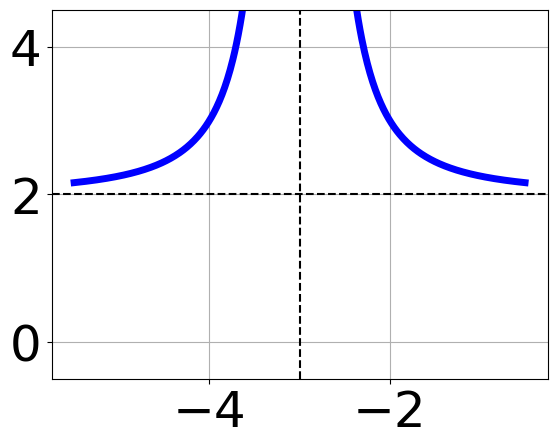
\includegraphics[width=0.5\textwidth]{../Figures/rationalGraphToEquationCopyB.png}
\end{center}
\begin{enumerate}[label=\Alph*.]
\item \( f(x) = \frac{-1}{x + 3} - 5 \)
\item \( f(x) = \frac{-1}{(x + 3)^2} - 5 \)
\item \( f(x) = \frac{1}{x - 3} - 5 \)
\item \( f(x) = \frac{1}{(x - 3)^2} - 5 \)
\item \( \text{None of the above} \)

\end{enumerate} }
\litem{
Solve the rational equation below. Then, choose the interval(s) that the solution(s) belongs to.\[ \frac{6x}{-5x -4} + \frac{-7x^{2}}{-30x^{2} -49 x -20} = \frac{-2}{6x + 5} \]\begin{enumerate}[label=\Alph*.]
\item \( x \in [-1.07,-0.97] \)
\item \( x_1 \in [0.09, 0.72] \text{ and } x_2 \in [-1.6,-0.81] \)
\item \( x_1 \in [0.09, 0.72] \text{ and } x_2 \in [-0.82,-0.29] \)
\item \( x \in [-0.88,-0.27] \)
\item \( \text{All solutions lead to invalid or complex values in the equation.} \)

\end{enumerate} }
\litem{
Solve the rational equation below. Then, choose the interval(s) that the solution(s) belongs to.\[ \frac{2x}{4x + 4} + \frac{-6x^{2}}{-16x^{2} -40 x -24} = \frac{7}{-4x -6} \]\begin{enumerate}[label=\Alph*.]
\item \( x_1 \in [-1.73, -1.62] \text{ and } x_2 \in [-1.39,-1.19] \)
\item \( x \in [-1.37,-1.19] \)
\item \( x_1 \in [-1.73, -1.62] \text{ and } x_2 \in [-1.17,-0.52] \)
\item \( \text{All solutions lead to invalid or complex values in the equation.} \)
\item \( x \in [-1.58,-1.47] \)

\end{enumerate} }
\end{enumerate}

\end{document}